\chapter{Materiais e Métodos}

Para o análise de uma rede SAC e DDPG foram usado a linguagem de programação Python.
A linguagem Python tem como prioridade a legibilidade do código sobre a velocidade \cite{ascher1999learning}. 
As vastas bibliotecas e \textit{frameworks} proporcionados pelo Python faz dela uma ferramenta extraordinária para fins de aprendizado de máquina e análise de dados.

\section{ROS}

O sistema operacional de robôs (ROS) é uma \textit{framework} flexível para escrever \textit{software} para robôs.
o ROS \cite{pyo2015ros} é uma coleção de ferramentas e bibliotecas.
O ROS fornece serviços padrões de sistemas operacionais, tais como a abstração de \textit{hardware}, controle de dispositivos de baixo nível, mensagens entre processos e gerenciamento de pacotes.
O conjunto de processos do ROS execução são representados em arquitetura de grafos onde o processamento é realizado em nós que recebem e enviam mensagens como sensores, controle, estado, planejamento, atuador e outros.

Apesar da importância da baixa latência no controle de robôs, o ROS não é um sistema operacional em tempo real, embora seja possível integrar o ROS com códigos em tempo real. Essa falta do sistema de tempo real está sendo endereçada no desenvolvimento do ROS 2.0.

\section{Gazebo}

A simulação de robôs é uma ferramenta essencial em toda a caixa de ferramentas de um roboticista.
Um bom simulador faz possível se testar rapidamente algoritmos, desenhar robôs, e treinar sistemas com inteligência artificial usando cenários realistas.
Com o Gazebo \cite{fairchild2016ros} é possível simular estes ambientes facilmente e com a vantagem de ter uma comunidade ativa. Isso faz do Gazebo uma grande ferramenta na área de simulação de robótica. Na Figura \ref{fig:gazebo} é mostrado a simulação do robô Turtlebot3 Burger em um ambiente de 3D no simulador Gazebo.

\begin{figure}[H]
\caption{Turtlebot3 Burger na simulação do Gazebo}
\centerline{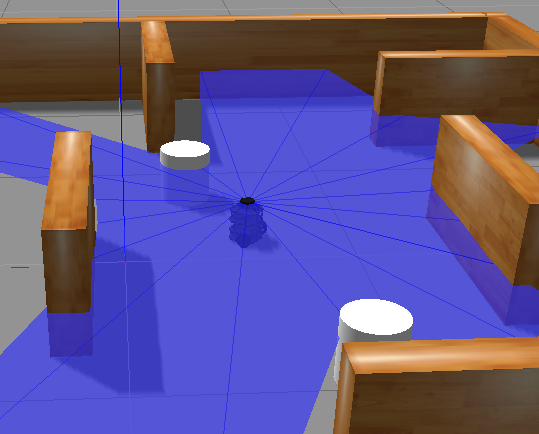
\includegraphics[width=\columnwidth]{imagens/gazebo.png}}
\small{Fonte: Autor}
\label{fig:gazebo}
\end{figure}

\section{Turtlebot}

O Turtlebot é uma robô de plataforma padrão ROS, e existem 3 versões da série.
Os Turtlebots são robôs móveis acessíveis e programáveis para o uso na educação, pesquisa, e \textit{hobbies} e prototipagem de produtos. A terceira versão foi usada no projeto e é mostrada na Figura \ref{fig:burger}.

\begin{figure}[H]
\caption{Turtlebot3 Burger real e simulado no Gazebo}
\centerline{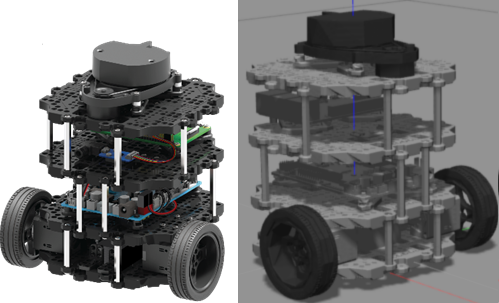
\includegraphics[width=\columnwidth]{imagens/burger.png}}
\small{Fonte: \cite{robotisemanual}}
\label{fig:burger}
\end{figure}

O Turtlebot3 Burger usa 2 motores DYNAMIXEL da série XL, para a detecção de objetos o Turtlebot3 utiliza um sensor \textit{laser} 360$^{\circ}$ LiDAR, e uma unidade de medição inercial (IMU) para o cálculo da odometria.
Todo o controle é feito pela placa controladora de código aberto OpenCR1.0 e o microprocessador Raspberry Pi 3.
A Tabela \ref{tab1} mostra todas as especificações de \textit{hardware} do Turtlebot3 versão Burger.

\begin{table}[H]
\caption{Especificação de Hardware do Turtlebot3 Burger}
\begin{center}
\begin{tabular}{l|l}
\hline
\textbf{Itens}&\textbf{Especificação} \\
\hline
Velocidade translacional máxima & 0.22 m/s \\
\hline
Velocidade rotacional máxima   & 2.84 rad/s (162.72$^{\circ}$/s) \\
\hline
Carga máxima                & 15kg \\ 
\hline
Tamanho (L x W x H)               & 138mm x 178mm x 192mm \\
\hline
Peso                        & 1kg \\
\hline
Limiar de escalada          & 10 mm ou mais baixo \\
\hline
Tempo de operação esperado       & 2h 30m \\
\hline
Tempo de espera para carregamento         & 2h 30m \\
\hline
Computador de Placa Única (SBC)   & Raspberry Pi 3 Model B e B+ \\
\hline
Atuador                       & DYNAMIXEL XL430-W250 \\
\hline
Sensor de Distância \textit{Laser} (LDS)     & 360 LDS-01 \\
\hline
IMU                            & \begin{tabular}[l]{@{}l@{}}Giroscópio 3 eixos\\ Acelerômetro 3 eixos\\ Magnetômetro 3 eixos\end{tabular} \\
\hline
Bateria                        & \begin{tabular}[l]{@{}l@{}}Polímero de lítio \\ 11.1V 1800mAh / 19.98Wh 5C \\ \end{tabular} \\
\hline

\end{tabular}
\label{tab1}
\end{center}
\small{Fonte: Adaptado de \cite{robotisemanual}}
\end{table}

\section{OpenCV}

\textit{Open Source Computer Vision} (OpenCV) é uma biblioteca de \textit{software} de código aberto para visão computacional e aprendizagem de máquina.
É principalmente usada para o desenvolver aplicações avançadas para processamento de imagem e visão compuacional (\citeauthor{bradski2008learning}, \citeyear{bradski2008learning}; \citeauthor{wang2010camera}, \citeyear{wang2010camera}).
OpenCV pode tirar quadros de um vídio e executar algoritmos para pegar informações necessárias.
Pode também identificar um objeto, reconhecer uma face ou rastrear o movimento de um objeto.
É comumente usado em aplicações de robótica \cite{oyama2009come}.

\section{Ambientes de Simulação}

Foram usados três ambientes para as simulações.
O primeiro ambiente é mostrado na Figura \ref{subfig:simulated_env1}, o ambiente representa uma área livre para o robô se mover.
As paredes do ambiente são as únicas coisas onde o agente pode colidir.
Se o robô móvel colidir com a parede ou qualquer obstáculo, uma recompensa negativa é dada para esta ação e o episódio atual termina.
O segundo ambiente é mostrado na Figura \ref{subfig:simulated_env2} e tem quatro obstáculos fixos.
Isso significa que este ambiente é mais complexo de um modo que o agente inteligente tem que fazer uma melhor estratégia para não colidir.
O terceiro ambiente, mostrado na Figura \ref{subfig:simulated_env3}, é mais complexo que os ambientes anteriores.
O número de paredes e obstáculos móveis, representados pelos blocos brancos, fazem o ambiente mais dinâmico, se aproximando de um ambiente no mundo real.

\begin{figure}[H]
\caption{Ambientes de treinamento usados na simulação do Gazebo}
    \begin{center}
    \begin{subfigure}[b]{0.3\textwidth}
        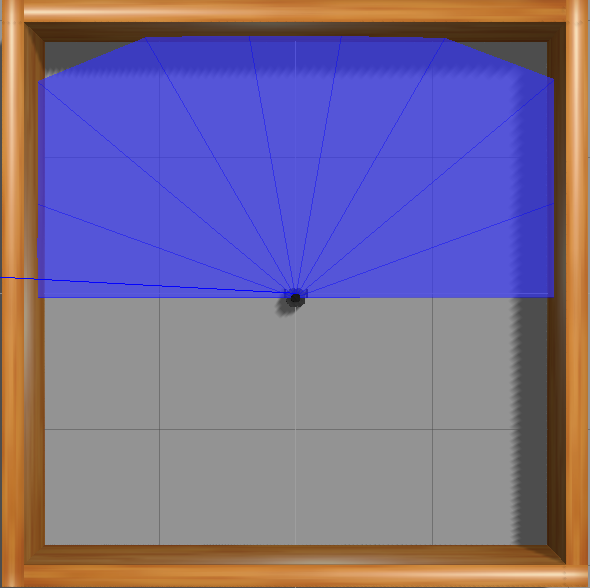
\includegraphics[width=\textwidth]{imagens/simulated_envs/amb1.png}
        \caption{Primeiro ambiente}
        \label{subfig:simulated_env1}
    \end{subfigure}
    ~ %add desired spacing between images, e. g. ~, \quad, \qquad, \hfill etc. 
      %(or a blank line to force the subfigure onto a new line)
    \begin{subfigure}[b]{0.3\textwidth}
        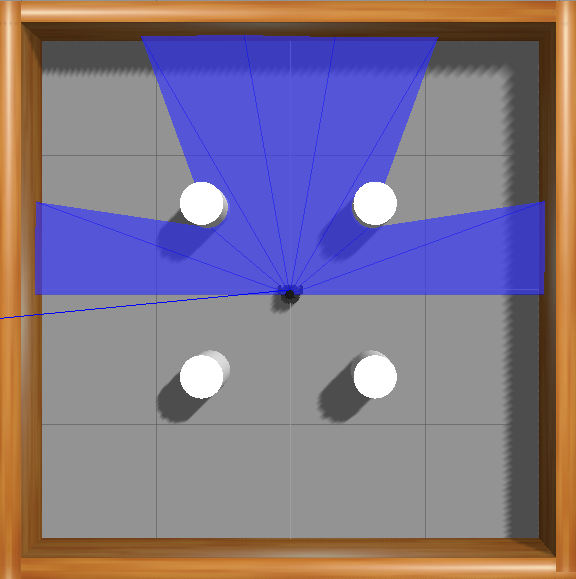
\includegraphics[width=\textwidth]{imagens/simulated_envs/amb2.png}
        \caption{Segundo ambiente}
        \label{subfig:simulated_env2}
    \end{subfigure}
    ~ %add desired spacing between images, e. g. ~, \quad, \qquad, \hfill etc. 
      %(or a blank line to force the subfigure onto a new line)
    \begin{subfigure}[b]{0.3\textwidth}
        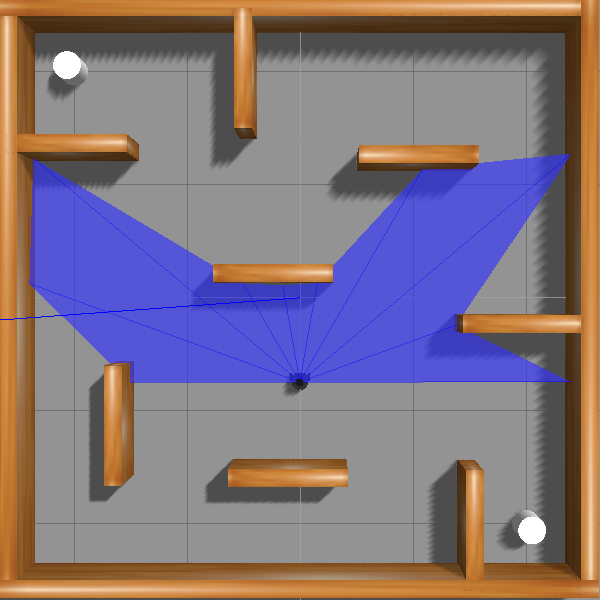
\includegraphics[width=\textwidth]{imagens/simulated_envs/amb3.png}
        \caption{Terceiro ambiente}
        \label{subfig:simulated_env3}
    \end{subfigure}\label{fig:environments}
    \end{center}
\small{Fonte: Autor}
\end{figure}

\section{Ambientes real}

Depois de treinar a rede DDPG e rede SAC por simulação, as redes serão testadas em um cenário real.
O Turtlebot3, versão Burger, será utilizado para executar estes testes.
Algumas das entradas necessárias das redes no ambiente real foram obtidas por processamento de imagem.
O primeiro ambiente real é mostrado na Figura \ref{subfig:real_env1} e se assemelha com o primeiro ambiente de simulação sem obstáculos.
O segundo ambiente real é mostrado na Figura z\ref{subfig:real_env2} e ele apresenta um ambiente complexo similar ao segundo e terceiro ambiente usado em simulação.

\begin{figure}[H]
\caption{Ambientes criados para testes da rede DDPG e rede SAC em ambiente real}
    \begin{center}
    \begin{subfigure}[b]{0.45\textwidth}
        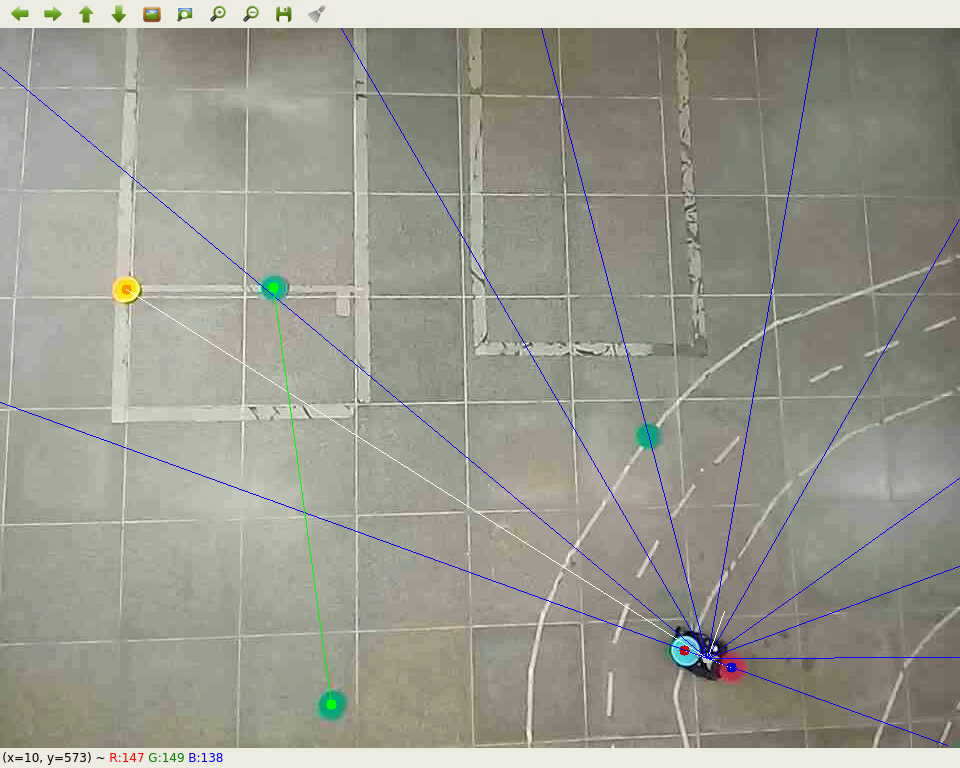
\includegraphics[width=\textwidth]{imagens/real_env1.png}
        \caption{Primeiro ambiente real}
        \label{subfig:real_env1}
    \end{subfigure}
    ~
    \begin{subfigure}[b]{0.45\textwidth}
        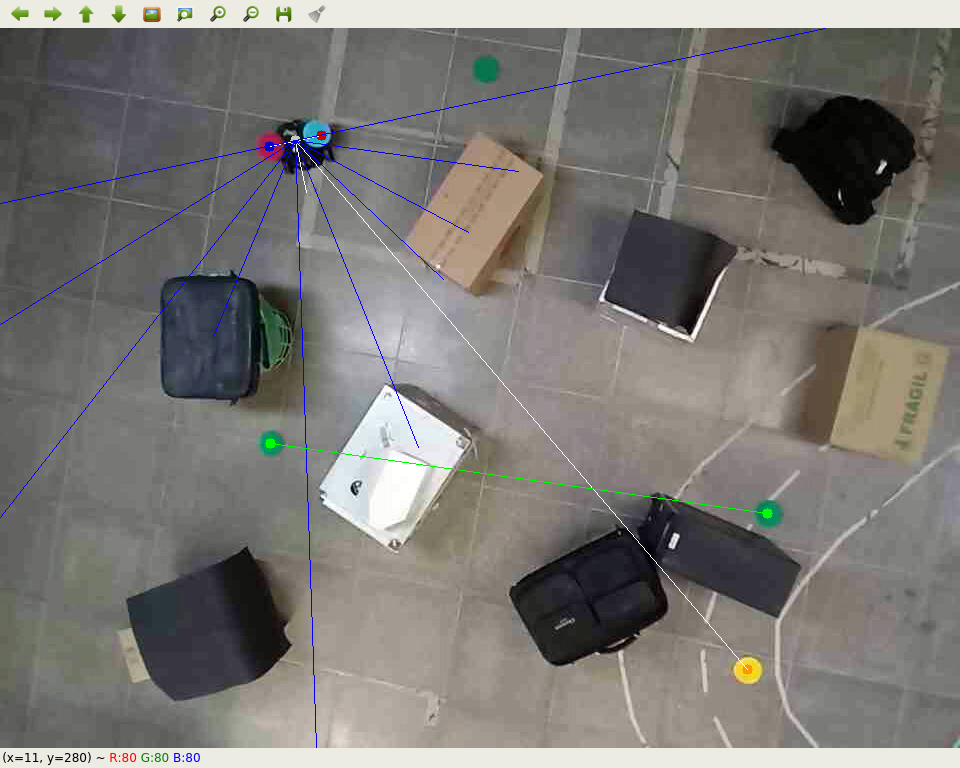
\includegraphics[width=\textwidth]{imagens/real_env2.png}
        \caption{Segundo ambiente real}
        \label{subfig:real_env2}
    \end{subfigure}
    \end{center}
    \label{fig:real_environments}
\small{Fonte: Autor}
\end{figure}

\section{Métodos}

A intenção deste trabalho é propor um sistema para um robô móvel em ordem de planejar seu movimento sem qualquer conhecimento do mapa no ambiente. Sua função de transição é definida como:
\begin{equation}
    v_t = f(x_t, p_t, v_{t-1})
\end{equation}

Onde $x_t$ é a observação da informação bruta do sensor, $p_t$ é a posição relativa do alvo em coordenadas polar, e $v_{t-1}$ é a velocidade do robô móvel no último intervalo de tempo.
Todas variáveis especificadas, anteriormente, podem ser definidas como o estado atual $s_t$ do robô móvel.
Na Figura \ref{fig:state_action} é mostrado o sistema de estados e ações que será utilizado nas redes para o treinamento.
Com esse modelo é possível retirar a ação que o robô fará, dado o seu estado atual.
Contudo, é preciso assegurar a frequência mínima de leitura dos dados de entrada para controlar o movimento do robô.
Pois se o robô tem uma leitura de frequência lenta das entradas, ele não pode reagir à um obstaculo na trajetória até o alvo.
Desde jeito, o robô pode reagir a novos estados rapidamente.
Esse método foi primeiro explorado por \cite{tai2017virtual}.

\begin{figure}[H]
\caption{Sistema de estados e ações}
\centerline{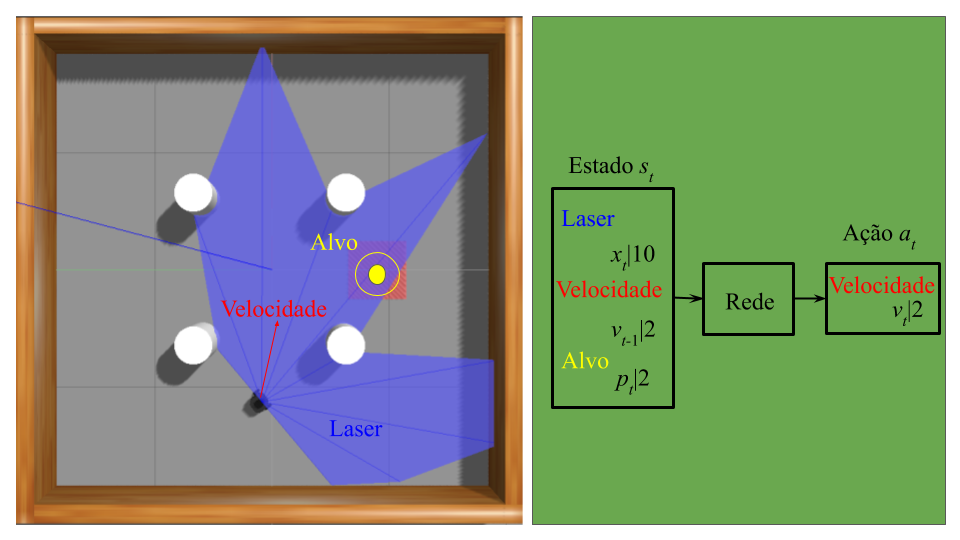
\includegraphics[width=\columnwidth]{imagens/state_action.png}}
\small{Fonte: Autor}
\label{fig:state_action}
\end{figure}

\subsection{Estruturas das Redes}

Uma vez que os sistema de estados e ações tenham sido definidos, é possível criar uma rede DDPG ou SAC para resolver o problema.
As redes têm como 14 entradas, como apresentado na Figura \ref{fig:in_out}, no qual 10 correspondem às leituras do \textit{laser} $x_t$, 2 correspondem à velocidade anterior linear $v_{t-1}$ e angular $\omega_{t-1}$, e 2 correspondem a posição relativa $d_t$ e ângulo $\theta_t$ do robô móvel ao alvo.
As amostras da leitura do sensor \textit{laser} são entre $-$90$^\circ$ e 90$^\circ$ em relação ao robô. A saída da rede é a ação de velocidade linear $v_t$ e angular $\omega_t$ que são aplicadas no robô móvel.

\begin{figure}[H]
\caption{Entradas e saídas da rede}
\centerline{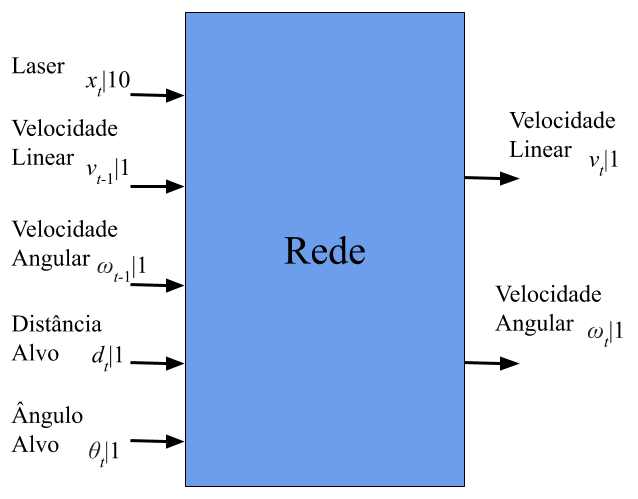
\includegraphics[width=10cm]{imagens/input_and_output.png}}
\small{Fonte: Autor}
\label{fig:in_out}
\end{figure}

A estrutura da rede DDPG é mostrada na Figura \ref{fig:ddpg_struct}. A rede ator tem como entrada o estado atual do robô móvel seguida por 3 camadas de redes neurais totalmente conectadas com 512 neurônios. A entrada da rede é transformada na velocidade linear e angular que serão os comandos enviados para os motores do robô móvel.
O intervalo da velocidade angular está restringindo entre $(-1,1)$ e a função de tangente hiperbólica $(tanh)$ é usada como função de ativação.
O intervalo da velocidade angular usou da função sigmóide como função de ativação para restringir a seus valores entre $(0,1)$.
Como não há leituras do sensor \textit{laser} na parte de trás do robô, a movimento de deslocamento de ré não é necessário.
As ações de saídas são então multiplicadas com os dois
hiperparâmetros que decidem a velocidade final linear e angular executada pelo robô móvel.
Para isso, foi usado como velocidade máxima linear $0.22$ $m/s$ e velocidade máxima angular $2$ $rad/s$ no robô Turtlebot3 versão Burger.
Na rede crítica, o valor de $Q$ do estado e ação atual são previstos.
Usando apenas 3 camadas de redes neurais totalmente conectadas para processar a entrada. Onde a ação, saída da rede ator, é concatenada na segunda camada de rede neural.
O valor de $Q$ é ativado através de uma função de ativação linear simples. Todas as respostas das funções de ativação citadas são mostradas na Figura \ref{fig:FA}.

\begin{figure}[H]
\caption{Estrutura do modelo da rede DDPG}
\centerline{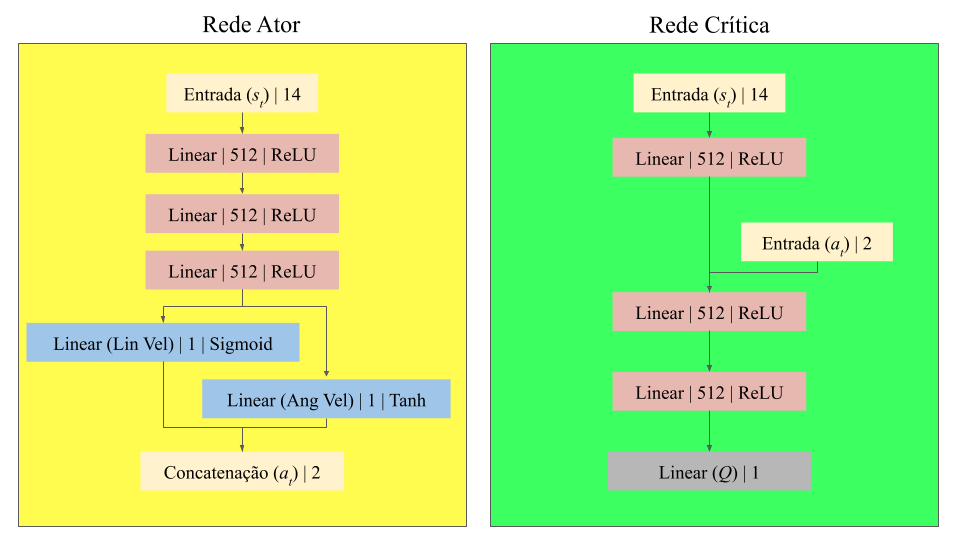
\includegraphics[width=\columnwidth]{imagens/ddpg_structure.png}}
\small{Fonte: Autor}
\label{fig:ddpg_struct}
\end{figure}

A estrutura da rede SAC é mostrada na Figura \ref{fig:sac_struct}.
A saída da rede ator tem o estado atual do robô móvel seguido por 4 camadas de redes neurais totalmente conectadas com 512 neurônios.
A entrada da rede é transformada nos comandos de velocidade angular e linear enviados para o robô móvel, do mesmo jeito que ocorre na rede ator da DDPG.
O intervalo de ação é restringindo entre $(-1,1)$ pela função de ativação de tangente hiperbólica. 
E as saídas da ação são mudados para a velocidade linear que varia entre $0$ até $0.22$ $m/s$ e a velocidade angular é entre $-2$ até $2$ $rad/s$ no Turtlebot3.
Já como diferença da rede DDPG, a rede SAC apresenta uma rede crítica que prediz o valor de $Q$ e uma rede de valor $V$ que prediz o valor do estado atual.
As duas redes usam apenas 2 camadas totalmente conectadas para processar o estado de entrada.

\begin{figure}[H]
\caption{Estrutura do modelo da rede SAC}
\centerline{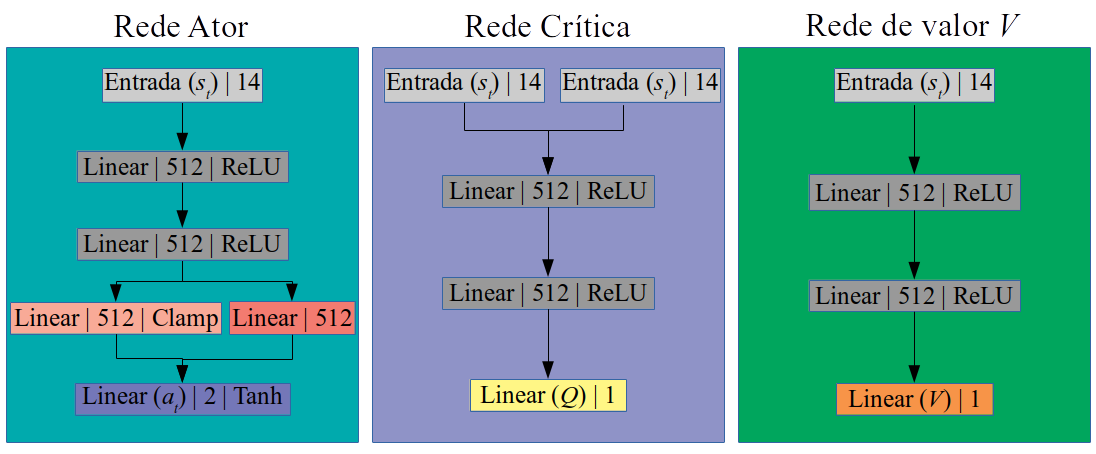
\includegraphics[width=\columnwidth]{imagens/sac_structure.png}}
\small{Fonte: Autor}
\label{fig:sac_struct}
\end{figure}

\subsection{Função de Recompensa}

Uma vez que o ambiente seja definido, é possível simular um robô móvel controlado para a tarefa de navegação.
É necessário definir o sistema recompensa e penalidade para a rede DDPG e SAC.
Lembrando que as recompensas e penalidades são números atribuídos passados para o agente inteligente.
Através disso, a rede vai fazer a propagação desses dados para seus pesos e bias em ordem para aprender os hiperparâmetros.

Existem quatro diferente condições para o sistema de recompensa que apresentaram melhores resultados para a resolução do problema e são os seguintes:

\begin{equation}
r (s_t, a_t) = 
\begin{cases}
r_{alcan\textit{ç}a} \ \textrm{se} \ d_t < c_d
\\
r_{colis\tilde{a}o} \ \textrm{se}\ min_x < c_o
\\
c_{r1}(d_{t-1} - d_t) \ \textrm{se} \ (d_{t-1} - d_t) > 0
\\
c_{r2} \ \textrm{se} \ (d_{t-1} - d_t) \leq 0
\end{cases}
\label{eq:r_function}
\end{equation}

Na Equação \ref{eq:r_function}, se o robô chega ao algo através da verificação de limite de distância $c_d$, uma recompensa positiva $(r_{alcan\textit{ç}a})$ é dada, mas se o robô colidir com um obstáculo através da verificação das leituras de alcance mínimo, uma recompensa negativa $(r_{colis\tilde{a}o})$ é dada.
Ambas as condições são suficientes para terminar o episódio de treino.
Ao contrário disso, a recompensa é baseada na diferença de distância do alvo comparado ao último intervalo de tempo $(d_{t-1} - d_t)$.
Se essa diferença é positiva a recompensa dada é a distância percorrida multiplicada pelo hiperparâmetro $(c_{r1})$, e se a a distância é negativa é usado o hiperparâmetro $(c_{r2})$.
Isso motiva o robô móvel a chegar mais próximo à posição do alvo e encoraja o agente a evitar obstáculo no ambiente.

\subsection{Positioning capture in real environments}

% % 
% % 
% % 
% estoy aqyu%%%%%%%%

After training the DDPG network through simulation, it will be tested in a real scenario.
The Turtlebot3, version Burger, will be used to perform this test.
It will be necessary to obtain the angle and distance of a target for the network to complete its goal.
So it was setup a camera in the ceiling to extract this information.

Firstly, the essential points positions to extract the angle and distance are taken from the image.
These positions include the target, left and right side of the robot, and three points to be a distance reference parameter.
Figure \ref{fig:pixel_to_meter} shows a frame of the scenario in which there were used different colored circles to identify the relevant points.
The yellow circle was attached as the target, the blue to the left side of the robot, the red to the right side and the three green circles were used as reference parameter to calculate the distance.

\begin{figure}[H]
\centerline{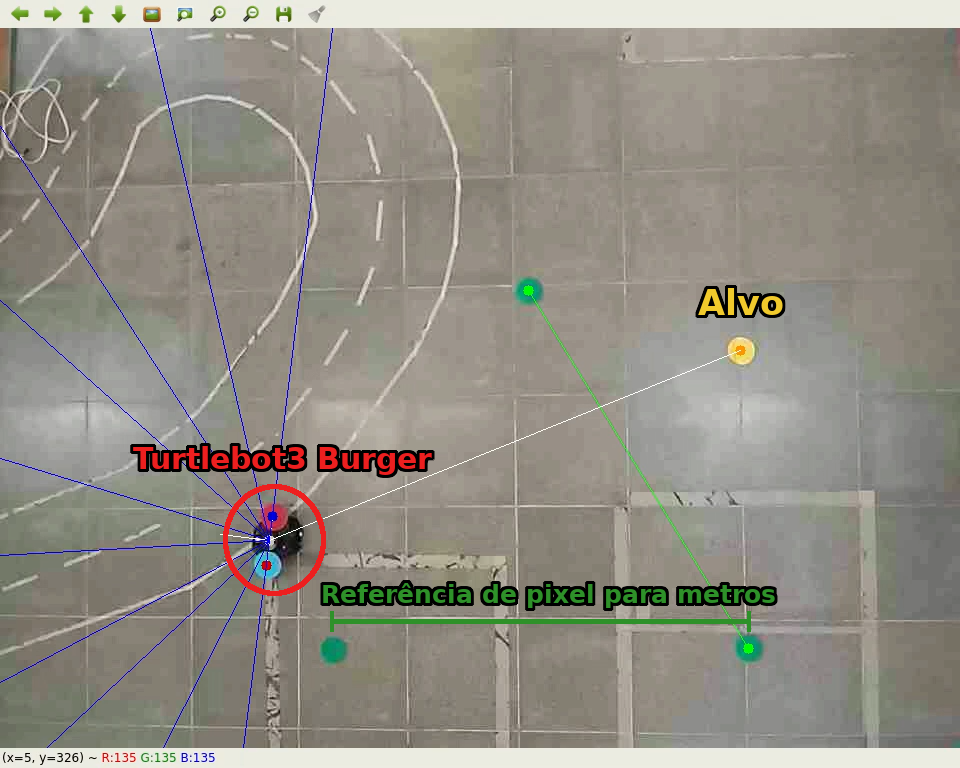
\includegraphics[width=10cm]{imagens/pixel_to_meter.png}}
\caption{Real environment relevant points}
\label{fig:pixel_to_meter}
\end{figure}


After the points were extracted from the center of the circles, it is possible to calculate the two necessary DDPG network inputs.
So, it is necessary to figure out the vector distance that connects the center of the Turtlebot3 to the target point, and the vector direction which represents the direction of the robot.
% Firstly, it is needed to compute the vector $distance$.
% It starts from the center of the Turtlebot3, which is equal to the midpoint of the blue and red points.
% The center of green circles have a predefined distance from each other, that helps to calculate the robot and target distance, doing by converting the module of vector $distance$ in pixels to the distance in meters.
% In other words, the actual distance between target and robot is estimated by comparing the pixels of the norm of the vector $distance$ with the pixels from the norm of the vector that connects the green circles, which real distance is already known. 
% %direction vector   
% The vector $direction$, like the $distance$, starts from the center of the Turtlebot3.
% With the blue and red circles that are on left and right sides of the mobile robot, respectively, it is possible to determine the direction of the robot's front, represented as vector $direction$.
% It is calculated by extracting the perpendicular vector to the vector which goes from the blue circle center to the red circle center.
% Now that we have the direction of Turtlebot3, it is possible to extract the angle between vector $distance$ and vector $direction$, which is the angle between the target and the front of the mobile robot.
% Finally, the two necessary information needed was obtained.
The distance and angle between the mobile robot and the target are calculated frame by frame, and it is used as the necessary inputs of the DDPG network simultaneously.



%aqui vou escrever mais 
%The center of green circles have a predefined distance from each other, what permits the calculation of robot and target distance by converting the pixel distance of the image to the distance in meters.
%aqui tbm





%After the points were extracted from the center of the circles, it is possible to calculate the two necessary DDPG network inputs.
%So, it is necessary to figure out the vector $distance$ that connects the center of Turtlebot3 to the target point, and the vector $direction$ which represents the direction of robot.
%The vector $direction$ starts from the center of Turtlebot3, which is equal to the midpoint of the blue and red points.
%The blue and red circles are on left and right sides of the mobile robot, respectively.
%With this it is possible to determine the front of the robot.

%aqui vou escrever mais 
%The center of green circles have a predefined distance from each other, what permits the calculation of robot and target distance by converting the pixel distance of the image to the distance in meters.
%aqui tbm